% Created by tikzDevice version 0.12.3.1 on 2021-07-04 23:14:39
% !TEX encoding = UTF-8 Unicode
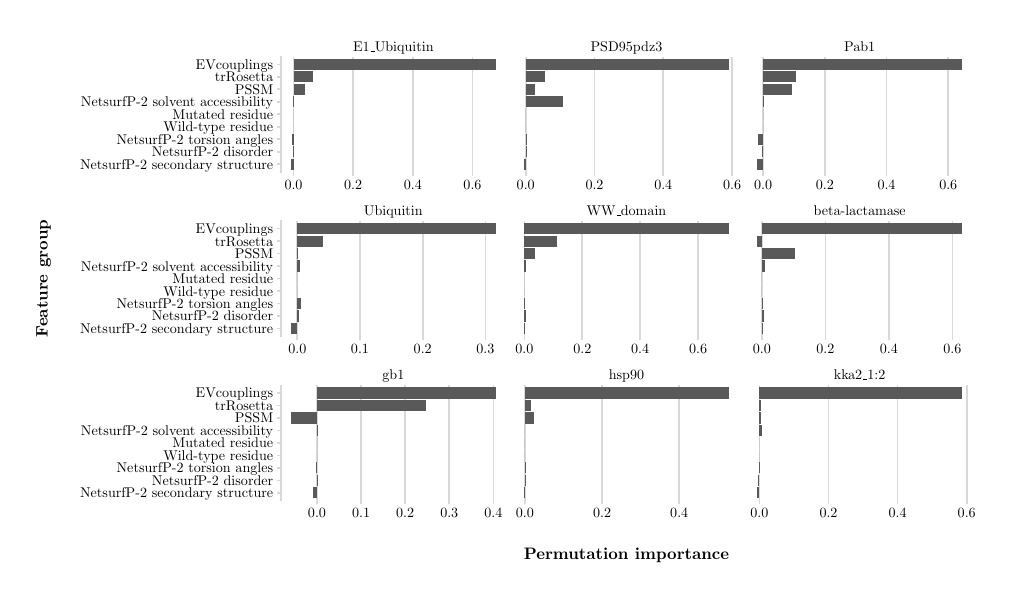
\begin{tikzpicture}[x=1pt,y=1pt]
\definecolor{fillColor}{RGB}{255,255,255}
\path[use as bounding box,fill=fillColor,fill opacity=0.00] (0,0) rectangle (344.26,196.49);
\begin{scope}
\path[clip] ( 91.51,144.44) rectangle (172.76,185.94);
\definecolor{drawColor}{gray}{0.85}

\path[draw=drawColor,line width= 0.6pt,line join=round] ( 96.07,144.44) --
	( 96.07,185.94);

\path[draw=drawColor,line width= 0.6pt,line join=round] (117.62,144.44) --
	(117.62,185.94);

\path[draw=drawColor,line width= 0.6pt,line join=round] (139.18,144.44) --
	(139.18,185.94);

\path[draw=drawColor,line width= 0.6pt,line join=round] (160.73,144.44) --
	(160.73,185.94);
\definecolor{fillColor}{gray}{0.35}

\path[fill=fillColor] ( 96.07,176.70) rectangle (102.95,180.76);

\path[fill=fillColor] ( 96.07,172.18) rectangle (100.18,176.24);

\path[fill=fillColor] ( 95.85,167.67) rectangle ( 96.07,171.73);

\path[fill=fillColor] ( 95.20,145.12) rectangle ( 96.07,149.18);

\path[fill=fillColor] ( 96.03,149.63) rectangle ( 96.07,153.69);

\path[fill=fillColor] ( 95.37,154.14) rectangle ( 96.07,158.20);

\path[fill=fillColor] ( 96.07,181.21) rectangle (169.06,185.27);

\path[fill=fillColor] ( 96.07,158.65) rectangle ( 96.07,162.71);

\path[fill=fillColor] ( 96.07,163.16) rectangle ( 96.07,167.22);
\end{scope}
\begin{scope}
\path[clip] ( 91.51, 85.06) rectangle (172.76,126.57);
\definecolor{drawColor}{gray}{0.85}

\path[draw=drawColor,line width= 0.6pt,line join=round] ( 97.43, 85.06) --
	( 97.43,126.57);

\path[draw=drawColor,line width= 0.6pt,line join=round] (120.09, 85.06) --
	(120.09,126.57);

\path[draw=drawColor,line width= 0.6pt,line join=round] (142.75, 85.06) --
	(142.75,126.57);

\path[draw=drawColor,line width= 0.6pt,line join=round] (165.40, 85.06) --
	(165.40,126.57);
\definecolor{fillColor}{gray}{0.35}

\path[fill=fillColor] ( 97.43,117.32) rectangle (106.63,121.38);

\path[fill=fillColor] ( 97.43,112.81) rectangle ( 97.45,116.87);

\path[fill=fillColor] ( 97.43,108.30) rectangle ( 98.36,112.36);

\path[fill=fillColor] ( 95.20, 85.74) rectangle ( 97.43, 89.80);

\path[fill=fillColor] ( 97.43, 90.25) rectangle ( 98.18, 94.31);

\path[fill=fillColor] ( 97.43, 94.76) rectangle ( 98.59, 98.82);

\path[fill=fillColor] ( 97.43,121.83) rectangle (169.06,125.89);

\path[fill=fillColor] ( 97.43, 99.28) rectangle ( 97.43,103.34);

\path[fill=fillColor] ( 97.43,103.79) rectangle ( 97.43,107.85);
\end{scope}
\begin{scope}
\path[clip] ( 91.51, 25.69) rectangle (172.76, 67.19);
\definecolor{drawColor}{gray}{0.85}

\path[draw=drawColor,line width= 0.6pt,line join=round] (104.55, 25.69) --
	(104.55, 67.19);

\path[draw=drawColor,line width= 0.6pt,line join=round] (120.48, 25.69) --
	(120.48, 67.19);

\path[draw=drawColor,line width= 0.6pt,line join=round] (136.42, 25.69) --
	(136.42, 67.19);

\path[draw=drawColor,line width= 0.6pt,line join=round] (152.35, 25.69) --
	(152.35, 67.19);

\path[draw=drawColor,line width= 0.6pt,line join=round] (168.29, 25.69) --
	(168.29, 67.19);
\definecolor{fillColor}{gray}{0.35}

\path[fill=fillColor] (104.55, 57.95) rectangle (143.92, 62.01);

\path[fill=fillColor] ( 95.20, 53.43) rectangle (104.55, 57.49);

\path[fill=fillColor] (104.55, 48.92) rectangle (104.87, 52.98);

\path[fill=fillColor] (103.14, 26.37) rectangle (104.55, 30.43);

\path[fill=fillColor] (104.47, 30.88) rectangle (104.55, 34.94);

\path[fill=fillColor] (104.18, 35.39) rectangle (104.55, 39.45);

\path[fill=fillColor] (104.55, 62.46) rectangle (169.06, 66.52);

\path[fill=fillColor] (104.55, 39.90) rectangle (104.55, 43.96);

\path[fill=fillColor] (104.55, 44.41) rectangle (104.55, 48.47);
\end{scope}
\begin{scope}
\path[clip] (175.76,144.44) rectangle (257.01,185.94);
\definecolor{drawColor}{gray}{0.85}

\path[draw=drawColor,line width= 0.6pt,line join=round] (179.98,144.44) --
	(179.98,185.94);

\path[draw=drawColor,line width= 0.6pt,line join=round] (204.83,144.44) --
	(204.83,185.94);

\path[draw=drawColor,line width= 0.6pt,line join=round] (229.68,144.44) --
	(229.68,185.94);

\path[draw=drawColor,line width= 0.6pt,line join=round] (254.53,144.44) --
	(254.53,185.94);
\definecolor{fillColor}{gray}{0.35}

\path[fill=fillColor] (179.98,176.70) rectangle (186.80,180.76);

\path[fill=fillColor] (179.98,172.18) rectangle (183.33,176.24);

\path[fill=fillColor] (179.98,167.67) rectangle (193.38,171.73);

\path[fill=fillColor] (179.45,145.12) rectangle (179.98,149.18);

\path[fill=fillColor] (179.91,149.63) rectangle (179.98,153.69);

\path[fill=fillColor] (179.97,154.14) rectangle (179.98,158.20);

\path[fill=fillColor] (179.98,181.21) rectangle (253.32,185.27);

\path[fill=fillColor] (179.98,158.65) rectangle (179.98,162.71);

\path[fill=fillColor] (179.98,163.16) rectangle (179.98,167.22);
\end{scope}
\begin{scope}
\path[clip] (175.76, 85.06) rectangle (257.01,126.57);
\definecolor{drawColor}{gray}{0.85}

\path[draw=drawColor,line width= 0.6pt,line join=round] (179.50, 85.06) --
	(179.50,126.57);

\path[draw=drawColor,line width= 0.6pt,line join=round] (200.42, 85.06) --
	(200.42,126.57);

\path[draw=drawColor,line width= 0.6pt,line join=round] (221.33, 85.06) --
	(221.33,126.57);

\path[draw=drawColor,line width= 0.6pt,line join=round] (242.25, 85.06) --
	(242.25,126.57);
\definecolor{fillColor}{gray}{0.35}

\path[fill=fillColor] (179.50,117.32) rectangle (191.28,121.38);

\path[fill=fillColor] (179.50,112.81) rectangle (183.24,116.87);

\path[fill=fillColor] (179.50,108.30) rectangle (180.15,112.36);

\path[fill=fillColor] (179.45, 85.74) rectangle (179.50, 89.80);

\path[fill=fillColor] (179.50, 90.25) rectangle (180.00, 94.31);

\path[fill=fillColor] (179.50, 94.76) rectangle (179.64, 98.82);

\path[fill=fillColor] (179.50,121.83) rectangle (253.32,125.89);

\path[fill=fillColor] (179.50, 99.28) rectangle (179.50,103.34);

\path[fill=fillColor] (179.50,103.79) rectangle (179.50,107.85);
\end{scope}
\begin{scope}
\path[clip] (175.76, 25.69) rectangle (257.01, 67.19);
\definecolor{drawColor}{gray}{0.85}

\path[draw=drawColor,line width= 0.6pt,line join=round] (179.65, 25.69) --
	(179.65, 67.19);

\path[draw=drawColor,line width= 0.6pt,line join=round] (207.55, 25.69) --
	(207.55, 67.19);

\path[draw=drawColor,line width= 0.6pt,line join=round] (235.44, 25.69) --
	(235.44, 67.19);
\definecolor{fillColor}{gray}{0.35}

\path[fill=fillColor] (179.65, 57.95) rectangle (182.04, 62.01);

\path[fill=fillColor] (179.65, 53.43) rectangle (183.02, 57.49);

\path[fill=fillColor] (179.65, 48.92) rectangle (179.65, 52.98);

\path[fill=fillColor] (179.45, 26.37) rectangle (179.65, 30.43);

\path[fill=fillColor] (179.65, 30.88) rectangle (179.84, 34.94);

\path[fill=fillColor] (179.65, 35.39) rectangle (179.80, 39.45);

\path[fill=fillColor] (179.65, 62.46) rectangle (253.32, 66.52);

\path[fill=fillColor] (179.65, 39.90) rectangle (179.65, 43.96);

\path[fill=fillColor] (179.65, 44.41) rectangle (179.65, 48.47);
\end{scope}
\begin{scope}
\path[clip] (260.01,144.44) rectangle (341.26,185.94);
\definecolor{drawColor}{gray}{0.85}

\path[draw=drawColor,line width= 0.6pt,line join=round] (265.75,144.44) --
	(265.75,185.94);

\path[draw=drawColor,line width= 0.6pt,line join=round] (288.05,144.44) --
	(288.05,185.94);

\path[draw=drawColor,line width= 0.6pt,line join=round] (310.35,144.44) --
	(310.35,185.94);

\path[draw=drawColor,line width= 0.6pt,line join=round] (332.66,144.44) --
	(332.66,185.94);
\definecolor{fillColor}{gray}{0.35}

\path[fill=fillColor] (265.75,176.70) rectangle (277.64,180.76);

\path[fill=fillColor] (265.75,172.18) rectangle (276.24,176.24);

\path[fill=fillColor] (265.71,167.67) rectangle (265.75,171.73);

\path[fill=fillColor] (263.70,145.12) rectangle (265.75,149.18);

\path[fill=fillColor] (265.46,149.63) rectangle (265.75,153.69);

\path[fill=fillColor] (263.97,154.14) rectangle (265.75,158.20);

\path[fill=fillColor] (265.75,181.21) rectangle (337.57,185.27);

\path[fill=fillColor] (265.75,158.65) rectangle (265.75,162.71);

\path[fill=fillColor] (265.75,163.16) rectangle (265.75,167.22);
\end{scope}
\begin{scope}
\path[clip] (260.01, 85.06) rectangle (341.26,126.57);
\definecolor{drawColor}{gray}{0.85}

\path[draw=drawColor,line width= 0.6pt,line join=round] (265.30, 85.06) --
	(265.30,126.57);

\path[draw=drawColor,line width= 0.6pt,line join=round] (288.25, 85.06) --
	(288.25,126.57);

\path[draw=drawColor,line width= 0.6pt,line join=round] (311.20, 85.06) --
	(311.20,126.57);

\path[draw=drawColor,line width= 0.6pt,line join=round] (334.15, 85.06) --
	(334.15,126.57);
\definecolor{fillColor}{gray}{0.35}

\path[fill=fillColor] (263.70,117.32) rectangle (265.30,121.38);

\path[fill=fillColor] (265.30,112.81) rectangle (277.33,116.87);

\path[fill=fillColor] (265.30,108.30) rectangle (266.55,112.36);

\path[fill=fillColor] (265.30, 85.74) rectangle (265.56, 89.80);

\path[fill=fillColor] (265.30, 90.25) rectangle (265.93, 94.31);

\path[fill=fillColor] (265.30, 94.76) rectangle (265.32, 98.82);

\path[fill=fillColor] (265.30,121.83) rectangle (337.57,125.89);

\path[fill=fillColor] (265.30, 99.28) rectangle (265.30,103.34);

\path[fill=fillColor] (265.30,103.79) rectangle (265.30,107.85);
\end{scope}
\begin{scope}
\path[clip] (260.01, 25.69) rectangle (341.26, 67.19);
\definecolor{drawColor}{gray}{0.85}

\path[draw=drawColor,line width= 0.6pt,line join=round] (264.41, 25.69) --
	(264.41, 67.19);

\path[draw=drawColor,line width= 0.6pt,line join=round] (289.39, 25.69) --
	(289.39, 67.19);

\path[draw=drawColor,line width= 0.6pt,line join=round] (314.36, 25.69) --
	(314.36, 67.19);

\path[draw=drawColor,line width= 0.6pt,line join=round] (339.34, 25.69) --
	(339.34, 67.19);
\definecolor{fillColor}{gray}{0.35}

\path[fill=fillColor] (264.41, 57.95) rectangle (265.09, 62.01);

\path[fill=fillColor] (264.41, 53.43) rectangle (265.12, 57.49);

\path[fill=fillColor] (264.41, 48.92) rectangle (265.39, 52.98);

\path[fill=fillColor] (263.70, 26.37) rectangle (264.41, 30.43);

\path[fill=fillColor] (264.04, 30.88) rectangle (264.41, 34.94);

\path[fill=fillColor] (264.36, 35.39) rectangle (264.41, 39.45);

\path[fill=fillColor] (264.41, 62.46) rectangle (337.57, 66.52);

\path[fill=fillColor] (264.41, 39.90) rectangle (264.41, 43.96);

\path[fill=fillColor] (264.41, 44.41) rectangle (264.41, 48.47);
\end{scope}
\begin{scope}
\path[clip] ( 91.51, 67.19) rectangle (172.76, 74.74);
\definecolor{drawColor}{RGB}{0,0,0}

\node[text=drawColor,anchor=base,inner sep=0pt, outer sep=0pt, scale=  0.51] at (132.13, 69.19) {gb1};
\end{scope}
\begin{scope}
\path[clip] (175.76, 67.19) rectangle (257.01, 74.74);
\definecolor{drawColor}{RGB}{0,0,0}

\node[text=drawColor,anchor=base,inner sep=0pt, outer sep=0pt, scale=  0.51] at (216.38, 69.19) {hsp90};
\end{scope}
\begin{scope}
\path[clip] (260.01, 67.19) rectangle (341.26, 74.74);
\definecolor{drawColor}{RGB}{0,0,0}

\node[text=drawColor,anchor=base,inner sep=0pt, outer sep=0pt, scale=  0.51] at (300.64, 69.19) {kka2\_1:2};
\end{scope}
\begin{scope}
\path[clip] ( 91.51,126.57) rectangle (172.76,134.11);
\definecolor{drawColor}{RGB}{0,0,0}

\node[text=drawColor,anchor=base,inner sep=0pt, outer sep=0pt, scale=  0.51] at (132.13,128.57) {Ubiquitin};
\end{scope}
\begin{scope}
\path[clip] (175.76,126.57) rectangle (257.01,134.11);
\definecolor{drawColor}{RGB}{0,0,0}

\node[text=drawColor,anchor=base,inner sep=0pt, outer sep=0pt, scale=  0.51] at (216.38,128.57) {WW\_domain};
\end{scope}
\begin{scope}
\path[clip] (260.01,126.57) rectangle (341.26,134.11);
\definecolor{drawColor}{RGB}{0,0,0}

\node[text=drawColor,anchor=base,inner sep=0pt, outer sep=0pt, scale=  0.51] at (300.64,128.57) {beta-lactamase};
\end{scope}
\begin{scope}
\path[clip] ( 91.51,185.94) rectangle (172.76,193.49);
\definecolor{drawColor}{RGB}{0,0,0}

\node[text=drawColor,anchor=base,inner sep=0pt, outer sep=0pt, scale=  0.51] at (132.13,187.94) {E1\_Ubiquitin};
\end{scope}
\begin{scope}
\path[clip] (175.76,185.94) rectangle (257.01,193.49);
\definecolor{drawColor}{RGB}{0,0,0}

\node[text=drawColor,anchor=base,inner sep=0pt, outer sep=0pt, scale=  0.51] at (216.38,187.94) {PSD95pdz3};
\end{scope}
\begin{scope}
\path[clip] (260.01,185.94) rectangle (341.26,193.49);
\definecolor{drawColor}{RGB}{0,0,0}

\node[text=drawColor,anchor=base,inner sep=0pt, outer sep=0pt, scale=  0.51] at (300.64,187.94) {Pab1};
\end{scope}
\begin{scope}
\path[clip] (  0.00,  0.00) rectangle (344.26,196.49);
\definecolor{drawColor}{gray}{0.85}

\path[draw=drawColor,line width= 0.6pt,line join=round] (104.55, 24.19) --
	(104.55, 25.69);

\path[draw=drawColor,line width= 0.6pt,line join=round] (120.48, 24.19) --
	(120.48, 25.69);

\path[draw=drawColor,line width= 0.6pt,line join=round] (136.42, 24.19) --
	(136.42, 25.69);

\path[draw=drawColor,line width= 0.6pt,line join=round] (152.35, 24.19) --
	(152.35, 25.69);

\path[draw=drawColor,line width= 0.6pt,line join=round] (168.29, 24.19) --
	(168.29, 25.69);
\end{scope}
\begin{scope}
\path[clip] (  0.00,  0.00) rectangle (344.26,196.49);
\definecolor{drawColor}{RGB}{0,0,0}

\node[text=drawColor,anchor=base,inner sep=0pt, outer sep=0pt, scale=  0.51] at (104.55, 19.36) {0.0};

\node[text=drawColor,anchor=base,inner sep=0pt, outer sep=0pt, scale=  0.51] at (120.48, 19.36) {0.1};

\node[text=drawColor,anchor=base,inner sep=0pt, outer sep=0pt, scale=  0.51] at (136.42, 19.36) {0.2};

\node[text=drawColor,anchor=base,inner sep=0pt, outer sep=0pt, scale=  0.51] at (152.35, 19.36) {0.3};

\node[text=drawColor,anchor=base,inner sep=0pt, outer sep=0pt, scale=  0.51] at (168.29, 19.36) {0.4};
\end{scope}
\begin{scope}
\path[clip] (  0.00,  0.00) rectangle (344.26,196.49);
\definecolor{drawColor}{gray}{0.85}

\path[draw=drawColor,line width= 0.6pt,line join=round] (179.65, 24.19) --
	(179.65, 25.69);

\path[draw=drawColor,line width= 0.6pt,line join=round] (207.55, 24.19) --
	(207.55, 25.69);

\path[draw=drawColor,line width= 0.6pt,line join=round] (235.44, 24.19) --
	(235.44, 25.69);
\end{scope}
\begin{scope}
\path[clip] (  0.00,  0.00) rectangle (344.26,196.49);
\definecolor{drawColor}{RGB}{0,0,0}

\node[text=drawColor,anchor=base,inner sep=0pt, outer sep=0pt, scale=  0.51] at (179.65, 19.36) {0.0};

\node[text=drawColor,anchor=base,inner sep=0pt, outer sep=0pt, scale=  0.51] at (207.55, 19.36) {0.2};

\node[text=drawColor,anchor=base,inner sep=0pt, outer sep=0pt, scale=  0.51] at (235.44, 19.36) {0.4};
\end{scope}
\begin{scope}
\path[clip] (  0.00,  0.00) rectangle (344.26,196.49);
\definecolor{drawColor}{gray}{0.85}

\path[draw=drawColor,line width= 0.6pt,line join=round] (264.41, 24.19) --
	(264.41, 25.69);

\path[draw=drawColor,line width= 0.6pt,line join=round] (289.39, 24.19) --
	(289.39, 25.69);

\path[draw=drawColor,line width= 0.6pt,line join=round] (314.36, 24.19) --
	(314.36, 25.69);

\path[draw=drawColor,line width= 0.6pt,line join=round] (339.34, 24.19) --
	(339.34, 25.69);
\end{scope}
\begin{scope}
\path[clip] (  0.00,  0.00) rectangle (344.26,196.49);
\definecolor{drawColor}{RGB}{0,0,0}

\node[text=drawColor,anchor=base,inner sep=0pt, outer sep=0pt, scale=  0.51] at (264.41, 19.36) {0.0};

\node[text=drawColor,anchor=base,inner sep=0pt, outer sep=0pt, scale=  0.51] at (289.39, 19.36) {0.2};

\node[text=drawColor,anchor=base,inner sep=0pt, outer sep=0pt, scale=  0.51] at (314.36, 19.36) {0.4};

\node[text=drawColor,anchor=base,inner sep=0pt, outer sep=0pt, scale=  0.51] at (339.34, 19.36) {0.6};
\end{scope}
\begin{scope}
\path[clip] (  0.00,  0.00) rectangle (344.26,196.49);
\definecolor{drawColor}{gray}{0.85}

\path[draw=drawColor,line width= 0.6pt,line join=round] ( 97.43, 83.56) --
	( 97.43, 85.06);

\path[draw=drawColor,line width= 0.6pt,line join=round] (120.09, 83.56) --
	(120.09, 85.06);

\path[draw=drawColor,line width= 0.6pt,line join=round] (142.75, 83.56) --
	(142.75, 85.06);

\path[draw=drawColor,line width= 0.6pt,line join=round] (165.40, 83.56) --
	(165.40, 85.06);
\end{scope}
\begin{scope}
\path[clip] (  0.00,  0.00) rectangle (344.26,196.49);
\definecolor{drawColor}{RGB}{0,0,0}

\node[text=drawColor,anchor=base,inner sep=0pt, outer sep=0pt, scale=  0.51] at ( 97.43, 78.74) {0.0};

\node[text=drawColor,anchor=base,inner sep=0pt, outer sep=0pt, scale=  0.51] at (120.09, 78.74) {0.1};

\node[text=drawColor,anchor=base,inner sep=0pt, outer sep=0pt, scale=  0.51] at (142.75, 78.74) {0.2};

\node[text=drawColor,anchor=base,inner sep=0pt, outer sep=0pt, scale=  0.51] at (165.40, 78.74) {0.3};
\end{scope}
\begin{scope}
\path[clip] (  0.00,  0.00) rectangle (344.26,196.49);
\definecolor{drawColor}{gray}{0.85}

\path[draw=drawColor,line width= 0.6pt,line join=round] (179.50, 83.56) --
	(179.50, 85.06);

\path[draw=drawColor,line width= 0.6pt,line join=round] (200.42, 83.56) --
	(200.42, 85.06);

\path[draw=drawColor,line width= 0.6pt,line join=round] (221.33, 83.56) --
	(221.33, 85.06);

\path[draw=drawColor,line width= 0.6pt,line join=round] (242.25, 83.56) --
	(242.25, 85.06);
\end{scope}
\begin{scope}
\path[clip] (  0.00,  0.00) rectangle (344.26,196.49);
\definecolor{drawColor}{RGB}{0,0,0}

\node[text=drawColor,anchor=base,inner sep=0pt, outer sep=0pt, scale=  0.51] at (179.50, 78.74) {0.0};

\node[text=drawColor,anchor=base,inner sep=0pt, outer sep=0pt, scale=  0.51] at (200.42, 78.74) {0.2};

\node[text=drawColor,anchor=base,inner sep=0pt, outer sep=0pt, scale=  0.51] at (221.33, 78.74) {0.4};

\node[text=drawColor,anchor=base,inner sep=0pt, outer sep=0pt, scale=  0.51] at (242.25, 78.74) {0.6};
\end{scope}
\begin{scope}
\path[clip] (  0.00,  0.00) rectangle (344.26,196.49);
\definecolor{drawColor}{gray}{0.85}

\path[draw=drawColor,line width= 0.6pt,line join=round] (265.30, 83.56) --
	(265.30, 85.06);

\path[draw=drawColor,line width= 0.6pt,line join=round] (288.25, 83.56) --
	(288.25, 85.06);

\path[draw=drawColor,line width= 0.6pt,line join=round] (311.20, 83.56) --
	(311.20, 85.06);

\path[draw=drawColor,line width= 0.6pt,line join=round] (334.15, 83.56) --
	(334.15, 85.06);
\end{scope}
\begin{scope}
\path[clip] (  0.00,  0.00) rectangle (344.26,196.49);
\definecolor{drawColor}{RGB}{0,0,0}

\node[text=drawColor,anchor=base,inner sep=0pt, outer sep=0pt, scale=  0.51] at (265.30, 78.74) {0.0};

\node[text=drawColor,anchor=base,inner sep=0pt, outer sep=0pt, scale=  0.51] at (288.25, 78.74) {0.2};

\node[text=drawColor,anchor=base,inner sep=0pt, outer sep=0pt, scale=  0.51] at (311.20, 78.74) {0.4};

\node[text=drawColor,anchor=base,inner sep=0pt, outer sep=0pt, scale=  0.51] at (334.15, 78.74) {0.6};
\end{scope}
\begin{scope}
\path[clip] (  0.00,  0.00) rectangle (344.26,196.49);
\definecolor{drawColor}{gray}{0.85}

\path[draw=drawColor,line width= 0.6pt,line join=round] ( 96.07,142.94) --
	( 96.07,144.44);

\path[draw=drawColor,line width= 0.6pt,line join=round] (117.62,142.94) --
	(117.62,144.44);

\path[draw=drawColor,line width= 0.6pt,line join=round] (139.18,142.94) --
	(139.18,144.44);

\path[draw=drawColor,line width= 0.6pt,line join=round] (160.73,142.94) --
	(160.73,144.44);
\end{scope}
\begin{scope}
\path[clip] (  0.00,  0.00) rectangle (344.26,196.49);
\definecolor{drawColor}{RGB}{0,0,0}

\node[text=drawColor,anchor=base,inner sep=0pt, outer sep=0pt, scale=  0.51] at ( 96.07,138.11) {0.0};

\node[text=drawColor,anchor=base,inner sep=0pt, outer sep=0pt, scale=  0.51] at (117.62,138.11) {0.2};

\node[text=drawColor,anchor=base,inner sep=0pt, outer sep=0pt, scale=  0.51] at (139.18,138.11) {0.4};

\node[text=drawColor,anchor=base,inner sep=0pt, outer sep=0pt, scale=  0.51] at (160.73,138.11) {0.6};
\end{scope}
\begin{scope}
\path[clip] (  0.00,  0.00) rectangle (344.26,196.49);
\definecolor{drawColor}{gray}{0.85}

\path[draw=drawColor,line width= 0.6pt,line join=round] (179.98,142.94) --
	(179.98,144.44);

\path[draw=drawColor,line width= 0.6pt,line join=round] (204.83,142.94) --
	(204.83,144.44);

\path[draw=drawColor,line width= 0.6pt,line join=round] (229.68,142.94) --
	(229.68,144.44);

\path[draw=drawColor,line width= 0.6pt,line join=round] (254.53,142.94) --
	(254.53,144.44);
\end{scope}
\begin{scope}
\path[clip] (  0.00,  0.00) rectangle (344.26,196.49);
\definecolor{drawColor}{RGB}{0,0,0}

\node[text=drawColor,anchor=base,inner sep=0pt, outer sep=0pt, scale=  0.51] at (179.98,138.11) {0.0};

\node[text=drawColor,anchor=base,inner sep=0pt, outer sep=0pt, scale=  0.51] at (204.83,138.11) {0.2};

\node[text=drawColor,anchor=base,inner sep=0pt, outer sep=0pt, scale=  0.51] at (229.68,138.11) {0.4};

\node[text=drawColor,anchor=base,inner sep=0pt, outer sep=0pt, scale=  0.51] at (254.53,138.11) {0.6};
\end{scope}
\begin{scope}
\path[clip] (  0.00,  0.00) rectangle (344.26,196.49);
\definecolor{drawColor}{gray}{0.85}

\path[draw=drawColor,line width= 0.6pt,line join=round] (265.75,142.94) --
	(265.75,144.44);

\path[draw=drawColor,line width= 0.6pt,line join=round] (288.05,142.94) --
	(288.05,144.44);

\path[draw=drawColor,line width= 0.6pt,line join=round] (310.35,142.94) --
	(310.35,144.44);

\path[draw=drawColor,line width= 0.6pt,line join=round] (332.66,142.94) --
	(332.66,144.44);
\end{scope}
\begin{scope}
\path[clip] (  0.00,  0.00) rectangle (344.26,196.49);
\definecolor{drawColor}{RGB}{0,0,0}

\node[text=drawColor,anchor=base,inner sep=0pt, outer sep=0pt, scale=  0.51] at (265.75,138.11) {0.0};

\node[text=drawColor,anchor=base,inner sep=0pt, outer sep=0pt, scale=  0.51] at (288.05,138.11) {0.2};

\node[text=drawColor,anchor=base,inner sep=0pt, outer sep=0pt, scale=  0.51] at (310.35,138.11) {0.4};

\node[text=drawColor,anchor=base,inner sep=0pt, outer sep=0pt, scale=  0.51] at (332.66,138.11) {0.6};
\end{scope}
\begin{scope}
\path[clip] (  0.00,  0.00) rectangle (344.26,196.49);
\definecolor{drawColor}{gray}{0.85}

\path[draw=drawColor,line width= 0.6pt,line join=round,line cap=rect] ( 91.51,144.44) --
	( 91.51,185.94);
\end{scope}
\begin{scope}
\path[clip] (  0.00,  0.00) rectangle (344.26,196.49);
\definecolor{drawColor}{RGB}{0,0,0}

\node[text=drawColor,anchor=base east,inner sep=0pt, outer sep=0pt, scale=  0.51] at ( 88.72,145.38) {NetsurfP-2 secondary structure};

\node[text=drawColor,anchor=base east,inner sep=0pt, outer sep=0pt, scale=  0.51] at ( 88.72,149.89) {NetsurfP-2 disorder};

\node[text=drawColor,anchor=base east,inner sep=0pt, outer sep=0pt, scale=  0.51] at ( 88.72,154.40) {NetsurfP-2 torsion angles};

\node[text=drawColor,anchor=base east,inner sep=0pt, outer sep=0pt, scale=  0.51] at ( 88.72,158.91) {Wild-type residue};

\node[text=drawColor,anchor=base east,inner sep=0pt, outer sep=0pt, scale=  0.51] at ( 88.72,163.42) {Mutated residue};

\node[text=drawColor,anchor=base east,inner sep=0pt, outer sep=0pt, scale=  0.51] at ( 88.72,167.93) {NetsurfP-2 solvent accessibility};

\node[text=drawColor,anchor=base east,inner sep=0pt, outer sep=0pt, scale=  0.51] at ( 88.72,172.44) {PSSM};

\node[text=drawColor,anchor=base east,inner sep=0pt, outer sep=0pt, scale=  0.51] at ( 88.72,176.95) {trRosetta};

\node[text=drawColor,anchor=base east,inner sep=0pt, outer sep=0pt, scale=  0.51] at ( 88.72,181.47) {EVcouplings};
\end{scope}
\begin{scope}
\path[clip] (  0.00,  0.00) rectangle (344.26,196.49);
\definecolor{drawColor}{gray}{0.85}

\path[draw=drawColor,line width= 0.6pt,line join=round] ( 90.01,147.15) --
	( 91.51,147.15);

\path[draw=drawColor,line width= 0.6pt,line join=round] ( 90.01,151.66) --
	( 91.51,151.66);

\path[draw=drawColor,line width= 0.6pt,line join=round] ( 90.01,156.17) --
	( 91.51,156.17);

\path[draw=drawColor,line width= 0.6pt,line join=round] ( 90.01,160.68) --
	( 91.51,160.68);

\path[draw=drawColor,line width= 0.6pt,line join=round] ( 90.01,165.19) --
	( 91.51,165.19);

\path[draw=drawColor,line width= 0.6pt,line join=round] ( 90.01,169.70) --
	( 91.51,169.70);

\path[draw=drawColor,line width= 0.6pt,line join=round] ( 90.01,174.21) --
	( 91.51,174.21);

\path[draw=drawColor,line width= 0.6pt,line join=round] ( 90.01,178.73) --
	( 91.51,178.73);

\path[draw=drawColor,line width= 0.6pt,line join=round] ( 90.01,183.24) --
	( 91.51,183.24);
\end{scope}
\begin{scope}
\path[clip] (  0.00,  0.00) rectangle (344.26,196.49);
\definecolor{drawColor}{gray}{0.85}

\path[draw=drawColor,line width= 0.6pt,line join=round,line cap=rect] ( 91.51, 85.06) --
	( 91.51,126.57);
\end{scope}
\begin{scope}
\path[clip] (  0.00,  0.00) rectangle (344.26,196.49);
\definecolor{drawColor}{RGB}{0,0,0}

\node[text=drawColor,anchor=base east,inner sep=0pt, outer sep=0pt, scale=  0.51] at ( 88.72, 86.00) {NetsurfP-2 secondary structure};

\node[text=drawColor,anchor=base east,inner sep=0pt, outer sep=0pt, scale=  0.51] at ( 88.72, 90.51) {NetsurfP-2 disorder};

\node[text=drawColor,anchor=base east,inner sep=0pt, outer sep=0pt, scale=  0.51] at ( 88.72, 95.02) {NetsurfP-2 torsion angles};

\node[text=drawColor,anchor=base east,inner sep=0pt, outer sep=0pt, scale=  0.51] at ( 88.72, 99.53) {Wild-type residue};

\node[text=drawColor,anchor=base east,inner sep=0pt, outer sep=0pt, scale=  0.51] at ( 88.72,104.05) {Mutated residue};

\node[text=drawColor,anchor=base east,inner sep=0pt, outer sep=0pt, scale=  0.51] at ( 88.72,108.56) {NetsurfP-2 solvent accessibility};

\node[text=drawColor,anchor=base east,inner sep=0pt, outer sep=0pt, scale=  0.51] at ( 88.72,113.07) {PSSM};

\node[text=drawColor,anchor=base east,inner sep=0pt, outer sep=0pt, scale=  0.51] at ( 88.72,117.58) {trRosetta};

\node[text=drawColor,anchor=base east,inner sep=0pt, outer sep=0pt, scale=  0.51] at ( 88.72,122.09) {EVcouplings};
\end{scope}
\begin{scope}
\path[clip] (  0.00,  0.00) rectangle (344.26,196.49);
\definecolor{drawColor}{gray}{0.85}

\path[draw=drawColor,line width= 0.6pt,line join=round] ( 90.01, 87.77) --
	( 91.51, 87.77);

\path[draw=drawColor,line width= 0.6pt,line join=round] ( 90.01, 92.28) --
	( 91.51, 92.28);

\path[draw=drawColor,line width= 0.6pt,line join=round] ( 90.01, 96.79) --
	( 91.51, 96.79);

\path[draw=drawColor,line width= 0.6pt,line join=round] ( 90.01,101.31) --
	( 91.51,101.31);

\path[draw=drawColor,line width= 0.6pt,line join=round] ( 90.01,105.82) --
	( 91.51,105.82);

\path[draw=drawColor,line width= 0.6pt,line join=round] ( 90.01,110.33) --
	( 91.51,110.33);

\path[draw=drawColor,line width= 0.6pt,line join=round] ( 90.01,114.84) --
	( 91.51,114.84);

\path[draw=drawColor,line width= 0.6pt,line join=round] ( 90.01,119.35) --
	( 91.51,119.35);

\path[draw=drawColor,line width= 0.6pt,line join=round] ( 90.01,123.86) --
	( 91.51,123.86);
\end{scope}
\begin{scope}
\path[clip] (  0.00,  0.00) rectangle (344.26,196.49);
\definecolor{drawColor}{gray}{0.85}

\path[draw=drawColor,line width= 0.6pt,line join=round,line cap=rect] ( 91.51, 25.69) --
	( 91.51, 67.19);
\end{scope}
\begin{scope}
\path[clip] (  0.00,  0.00) rectangle (344.26,196.49);
\definecolor{drawColor}{RGB}{0,0,0}

\node[text=drawColor,anchor=base east,inner sep=0pt, outer sep=0pt, scale=  0.51] at ( 88.72, 26.62) {NetsurfP-2 secondary structure};

\node[text=drawColor,anchor=base east,inner sep=0pt, outer sep=0pt, scale=  0.51] at ( 88.72, 31.14) {NetsurfP-2 disorder};

\node[text=drawColor,anchor=base east,inner sep=0pt, outer sep=0pt, scale=  0.51] at ( 88.72, 35.65) {NetsurfP-2 torsion angles};

\node[text=drawColor,anchor=base east,inner sep=0pt, outer sep=0pt, scale=  0.51] at ( 88.72, 40.16) {Wild-type residue};

\node[text=drawColor,anchor=base east,inner sep=0pt, outer sep=0pt, scale=  0.51] at ( 88.72, 44.67) {Mutated residue};

\node[text=drawColor,anchor=base east,inner sep=0pt, outer sep=0pt, scale=  0.51] at ( 88.72, 49.18) {NetsurfP-2 solvent accessibility};

\node[text=drawColor,anchor=base east,inner sep=0pt, outer sep=0pt, scale=  0.51] at ( 88.72, 53.69) {PSSM};

\node[text=drawColor,anchor=base east,inner sep=0pt, outer sep=0pt, scale=  0.51] at ( 88.72, 58.20) {trRosetta};

\node[text=drawColor,anchor=base east,inner sep=0pt, outer sep=0pt, scale=  0.51] at ( 88.72, 62.72) {EVcouplings};
\end{scope}
\begin{scope}
\path[clip] (  0.00,  0.00) rectangle (344.26,196.49);
\definecolor{drawColor}{gray}{0.85}

\path[draw=drawColor,line width= 0.6pt,line join=round] ( 90.01, 28.40) --
	( 91.51, 28.40);

\path[draw=drawColor,line width= 0.6pt,line join=round] ( 90.01, 32.91) --
	( 91.51, 32.91);

\path[draw=drawColor,line width= 0.6pt,line join=round] ( 90.01, 37.42) --
	( 91.51, 37.42);

\path[draw=drawColor,line width= 0.6pt,line join=round] ( 90.01, 41.93) --
	( 91.51, 41.93);

\path[draw=drawColor,line width= 0.6pt,line join=round] ( 90.01, 46.44) --
	( 91.51, 46.44);

\path[draw=drawColor,line width= 0.6pt,line join=round] ( 90.01, 50.95) --
	( 91.51, 50.95);

\path[draw=drawColor,line width= 0.6pt,line join=round] ( 90.01, 55.46) --
	( 91.51, 55.46);

\path[draw=drawColor,line width= 0.6pt,line join=round] ( 90.01, 59.98) --
	( 91.51, 59.98);

\path[draw=drawColor,line width= 0.6pt,line join=round] ( 90.01, 64.49) --
	( 91.51, 64.49);
\end{scope}
\begin{scope}
\path[clip] (  0.00,  0.00) rectangle (344.26,196.49);
\definecolor{drawColor}{RGB}{0,0,0}

\node[text=drawColor,anchor=base,inner sep=0pt, outer sep=0pt, scale=  0.60] at (216.38,  4.17) {\bfseries Permutation importance};
\end{scope}
\begin{scope}
\path[clip] (  0.00,  0.00) rectangle (344.26,196.49);
\definecolor{drawColor}{RGB}{0,0,0}

\node[text=drawColor,rotate= 90.00,anchor=base,inner sep=0pt, outer sep=0pt, scale=  0.60] at (  7.19,105.82) {\bfseries Feature group};
\end{scope}
\end{tikzpicture}%
